\documentclass[twoside]{book}

% Packages required by doxygen
\usepackage{calc}
\usepackage{doxygen}
\usepackage{graphicx}
\usepackage[utf8]{inputenc}
\usepackage{makeidx}
\usepackage{multicol}
\usepackage{multirow}
\usepackage{textcomp}
\usepackage[table]{xcolor}

% Font selection
\usepackage[T1]{fontenc}
\usepackage{mathptmx}
\usepackage[scaled=.90]{helvet}
\usepackage{courier}
\usepackage{amssymb}
\usepackage{sectsty}
\renewcommand{\familydefault}{\sfdefault}
\allsectionsfont{%
  \fontseries{bc}\selectfont%
  \color{darkgray}%
}
\renewcommand{\DoxyLabelFont}{%
  \fontseries{bc}\selectfont%
  \color{darkgray}%
}

% Page & text layout
\usepackage{geometry}
\geometry{%
  a4paper,%
  top=2.5cm,%
  bottom=2.5cm,%
  left=2.5cm,%
  right=2.5cm%
}
\tolerance=750
\hfuzz=15pt
\hbadness=750
\setlength{\emergencystretch}{15pt}
\setlength{\parindent}{0cm}
\setlength{\parskip}{0.2cm}
\makeatletter
\renewcommand{\paragraph}{%
  \@startsection{paragraph}{4}{0ex}{-1.0ex}{1.0ex}{%
    \normalfont\normalsize\bfseries\SS@parafont%
  }%
}
\renewcommand{\subparagraph}{%
  \@startsection{subparagraph}{5}{0ex}{-1.0ex}{1.0ex}{%
    \normalfont\normalsize\bfseries\SS@subparafont%
  }%
}
\makeatother

% Headers & footers
\usepackage{fancyhdr}
\pagestyle{fancyplain}
\fancyhead[LE]{\fancyplain{}{\bfseries\thepage}}
\fancyhead[CE]{\fancyplain{}{}}
\fancyhead[RE]{\fancyplain{}{\bfseries\leftmark}}
\fancyhead[LO]{\fancyplain{}{\bfseries\rightmark}}
\fancyhead[CO]{\fancyplain{}{}}
\fancyhead[RO]{\fancyplain{}{\bfseries\thepage}}
\fancyfoot[LE]{\fancyplain{}{}}
\fancyfoot[CE]{\fancyplain{}{}}
\fancyfoot[RE]{\fancyplain{}{\bfseries\scriptsize Generated on Sat Jun 29 2019 10\-:28\-:49 for print\-\_\-ip by Doxygen }}
\fancyfoot[LO]{\fancyplain{}{\bfseries\scriptsize Generated on Sat Jun 29 2019 10\-:28\-:49 for print\-\_\-ip by Doxygen }}
\fancyfoot[CO]{\fancyplain{}{}}
\fancyfoot[RO]{\fancyplain{}{}}
\renewcommand{\footrulewidth}{0.4pt}
\renewcommand{\chaptermark}[1]{%
  \markboth{#1}{}%
}
\renewcommand{\sectionmark}[1]{%
  \markright{\thesection\ #1}%
}

% Indices & bibliography
\usepackage{natbib}
\usepackage[titles]{tocloft}
\setcounter{tocdepth}{3}
\setcounter{secnumdepth}{5}
\makeindex

% Hyperlinks (required, but should be loaded last)
\usepackage{ifpdf}
\ifpdf
  \usepackage[pdftex,pagebackref=true]{hyperref}
\else
  \usepackage[ps2pdf,pagebackref=true]{hyperref}
\fi
\hypersetup{%
  colorlinks=true,%
  linkcolor=blue,%
  citecolor=blue,%
  unicode%
}

% Custom commands
\newcommand{\clearemptydoublepage}{%
  \newpage{\pagestyle{empty}\cleardoublepage}%
}


%===== C O N T E N T S =====

\begin{document}

% Titlepage & ToC
\hypersetup{pageanchor=false}
\pagenumbering{roman}
\begin{titlepage}
\vspace*{7cm}
\begin{center}%
{\Large print\-\_\-ip }\\
\vspace*{1cm}
{\large Generated by Doxygen 1.8.6}\\
\vspace*{0.5cm}
{\small Sat Jun 29 2019 10:28:49}\\
\end{center}
\end{titlepage}
\clearemptydoublepage
\tableofcontents
\clearemptydoublepage
\pagenumbering{arabic}
\hypersetup{pageanchor=true}

%--- Begin generated contents ---
\chapter{Namespace Index}
\section{Namespace List}
Here is a list of all namespaces with brief descriptions\-:\begin{DoxyCompactList}
\item\contentsline{section}{\hyperlink{namespaceflaber}{flaber} }{\pageref{namespaceflaber}}{}
\end{DoxyCompactList}

\chapter{File Index}
\section{File List}
Here is a list of all files with brief descriptions\-:\begin{DoxyCompactList}
\item\contentsline{section}{src/\hyperlink{print__ip_8cpp}{print\-\_\-ip.\-cpp} }{\pageref{print__ip_8cpp}}{}
\item\contentsline{section}{src/\hyperlink{print__ip_8h}{print\-\_\-ip.\-h} }{\pageref{print__ip_8h}}{}
\end{DoxyCompactList}

\chapter{Namespace Documentation}
\hypertarget{namespaceflaber}{\section{flaber Namespace Reference}
\label{namespaceflaber}\index{flaber@{flaber}}
}
\subsection*{Functions}
\begin{DoxyCompactItemize}
\item 
{\footnotesize template$<$typename Char\-T $>$ }\\void \hyperlink{namespaceflaber_ac2e2220e0b43c7179450485776033a25}{print\-\_\-ip} (std\-::basic\-\_\-ostream$<$ Char\-T $>$ \&os, const std\-::basic\-\_\-string$<$ Char\-T $>$ \&ip)
\item 
{\footnotesize template$<$template$<$ typename, typename $>$ class Container\-T, typename Value\-T , typename Alloc\-T , typename  = std\-::enable\-\_\-if\-\_\-t$<$!is\-\_\-char\-\_\-v$<$\-Value\-T$>$, Value\-T$>$$>$ }\\void \hyperlink{namespaceflaber_a0a0f3ac76aaf479fde049bb26f0930ef}{print\-\_\-ip} (std\-::ostream \&os, const Container\-T$<$ Value\-T, Alloc\-T $>$ \&t)
\item 
{\footnotesize template$<$typename Char\-T , size\-\_\-t N$>$ }\\void \hyperlink{namespaceflaber_a899f2a8340371796390a26c56bd257c0}{print\-\_\-ip} (std\-::ostream \&os, Char\-T(\&arr)\mbox{[}N\mbox{]})
\item 
{\footnotesize template$<$class Int\-T , typename  = std\-::enable\-\_\-if\-\_\-t$<$std\-::is\-\_\-integral\-\_\-v$<$\-Int\-T$>$, Int\-T$>$$>$ }\\void \hyperlink{namespaceflaber_aa6c37128a4f8005fe33124a175e5df4e}{print\-\_\-ip} (std\-::ostream \&os, Int\-T ip)
\item 
{\footnotesize template$<$class... T\-Params$>$ }\\void \hyperlink{namespaceflaber_a2cd40a0efb0b9101246e8dcb11c6d18e}{print\-\_\-ip} (std\-::ostream \&os, const std\-::tuple$<$ T\-Params...$>$ \&tuple)
\end{DoxyCompactItemize}


\subsection{Function Documentation}
\hypertarget{namespaceflaber_ac2e2220e0b43c7179450485776033a25}{\index{flaber@{flaber}!print\-\_\-ip@{print\-\_\-ip}}
\index{print\-\_\-ip@{print\-\_\-ip}!flaber@{flaber}}
\subsubsection[{print\-\_\-ip}]{\setlength{\rightskip}{0pt plus 5cm}template$<$typename Char\-T $>$ void flaber\-::print\-\_\-ip (
\begin{DoxyParamCaption}
\item[{std\-::basic\-\_\-ostream$<$ Char\-T $>$ \&}]{os, }
\item[{const std\-::basic\-\_\-string$<$ Char\-T $>$ \&}]{ip}
\end{DoxyParamCaption}
)}}\label{namespaceflaber_ac2e2220e0b43c7179450485776033a25}
\hypertarget{namespaceflaber_a0a0f3ac76aaf479fde049bb26f0930ef}{\index{flaber@{flaber}!print\-\_\-ip@{print\-\_\-ip}}
\index{print\-\_\-ip@{print\-\_\-ip}!flaber@{flaber}}
\subsubsection[{print\-\_\-ip}]{\setlength{\rightskip}{0pt plus 5cm}template$<$template$<$ typename, typename $>$ class Container\-T, typename Value\-T , typename Alloc\-T , typename  = std\-::enable\-\_\-if\-\_\-t$<$!is\-\_\-char\-\_\-v$<$\-Value\-T$>$, Value\-T$>$$>$ void flaber\-::print\-\_\-ip (
\begin{DoxyParamCaption}
\item[{std\-::ostream \&}]{os, }
\item[{const Container\-T$<$ Value\-T, Alloc\-T $>$ \&}]{t}
\end{DoxyParamCaption}
)}}\label{namespaceflaber_a0a0f3ac76aaf479fde049bb26f0930ef}
\hypertarget{namespaceflaber_a899f2a8340371796390a26c56bd257c0}{\index{flaber@{flaber}!print\-\_\-ip@{print\-\_\-ip}}
\index{print\-\_\-ip@{print\-\_\-ip}!flaber@{flaber}}
\subsubsection[{print\-\_\-ip}]{\setlength{\rightskip}{0pt plus 5cm}template$<$typename Char\-T , size\-\_\-t N$>$ void flaber\-::print\-\_\-ip (
\begin{DoxyParamCaption}
\item[{std\-::ostream \&}]{os, }
\item[{Char\-T(\&)}]{arr\mbox{[}\-N\mbox{]}}
\end{DoxyParamCaption}
)}}\label{namespaceflaber_a899f2a8340371796390a26c56bd257c0}
\hypertarget{namespaceflaber_aa6c37128a4f8005fe33124a175e5df4e}{\index{flaber@{flaber}!print\-\_\-ip@{print\-\_\-ip}}
\index{print\-\_\-ip@{print\-\_\-ip}!flaber@{flaber}}
\subsubsection[{print\-\_\-ip}]{\setlength{\rightskip}{0pt plus 5cm}template$<$class Int\-T , typename  = std\-::enable\-\_\-if\-\_\-t$<$std\-::is\-\_\-integral\-\_\-v$<$\-Int\-T$>$, Int\-T$>$$>$ void flaber\-::print\-\_\-ip (
\begin{DoxyParamCaption}
\item[{std\-::ostream \&}]{os, }
\item[{Int\-T}]{ip}
\end{DoxyParamCaption}
)}}\label{namespaceflaber_aa6c37128a4f8005fe33124a175e5df4e}
\hypertarget{namespaceflaber_a2cd40a0efb0b9101246e8dcb11c6d18e}{\index{flaber@{flaber}!print\-\_\-ip@{print\-\_\-ip}}
\index{print\-\_\-ip@{print\-\_\-ip}!flaber@{flaber}}
\subsubsection[{print\-\_\-ip}]{\setlength{\rightskip}{0pt plus 5cm}template$<$class... T\-Params$>$ void flaber\-::print\-\_\-ip (
\begin{DoxyParamCaption}
\item[{std\-::ostream \&}]{os, }
\item[{const std\-::tuple$<$ T\-Params...$>$ \&}]{tuple}
\end{DoxyParamCaption}
)}}\label{namespaceflaber_a2cd40a0efb0b9101246e8dcb11c6d18e}

\chapter{File Documentation}
\hypertarget{print__ip_8cpp}{\section{src/print\-\_\-ip.cpp File Reference}
\label{print__ip_8cpp}\index{src/print\-\_\-ip.\-cpp@{src/print\-\_\-ip.\-cpp}}
}
{\ttfamily \#include $<$iostream$>$}\\*
{\ttfamily \#include $<$vector$>$}\\*
{\ttfamily \#include $<$list$>$}\\*
{\ttfamily \#include $<$tuple$>$}\\*
{\ttfamily \#include \char`\"{}print\-\_\-ip.\-h\char`\"{}}\\*
Include dependency graph for print\-\_\-ip.\-cpp\-:
\nopagebreak
\begin{figure}[H]
\begin{center}
\leavevmode
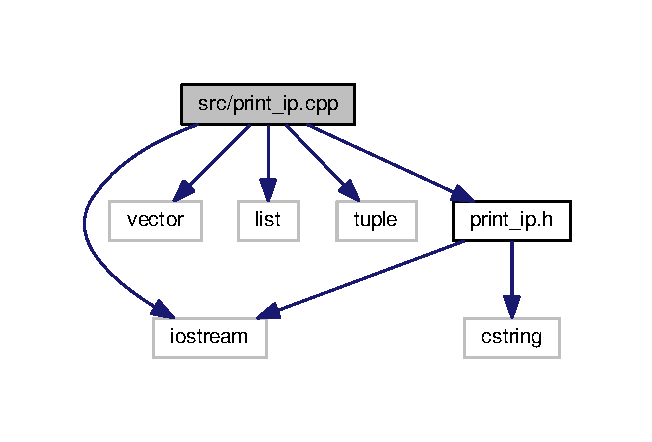
\includegraphics[width=313pt]{print__ip_8cpp__incl}
\end{center}
\end{figure}
\subsection*{Functions}
\begin{DoxyCompactItemize}
\item 
int \hyperlink{print__ip_8cpp_ae66f6b31b5ad750f1fe042a706a4e3d4}{main} ()
\end{DoxyCompactItemize}


\subsection{Function Documentation}
\hypertarget{print__ip_8cpp_ae66f6b31b5ad750f1fe042a706a4e3d4}{\index{print\-\_\-ip.\-cpp@{print\-\_\-ip.\-cpp}!main@{main}}
\index{main@{main}!print_ip.cpp@{print\-\_\-ip.\-cpp}}
\subsubsection[{main}]{\setlength{\rightskip}{0pt plus 5cm}int main (
\begin{DoxyParamCaption}
{}
\end{DoxyParamCaption}
)}}\label{print__ip_8cpp_ae66f6b31b5ad750f1fe042a706a4e3d4}

\hypertarget{print__ip_8h}{\section{src/print\-\_\-ip.h File Reference}
\label{print__ip_8h}\index{src/print\-\_\-ip.\-h@{src/print\-\_\-ip.\-h}}
}
{\ttfamily \#include $<$iostream$>$}\\*
{\ttfamily \#include $<$cstring$>$}\\*
Include dependency graph for print\-\_\-ip.\-h\-:
\nopagebreak
\begin{figure}[H]
\begin{center}
\leavevmode
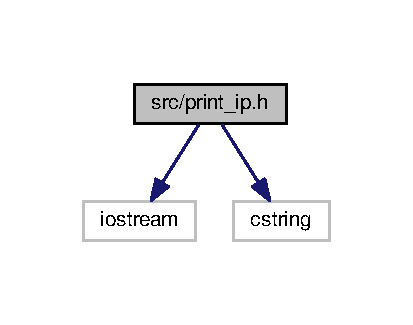
\includegraphics[width=198pt]{print__ip_8h__incl}
\end{center}
\end{figure}
This graph shows which files directly or indirectly include this file\-:
\nopagebreak
\begin{figure}[H]
\begin{center}
\leavevmode
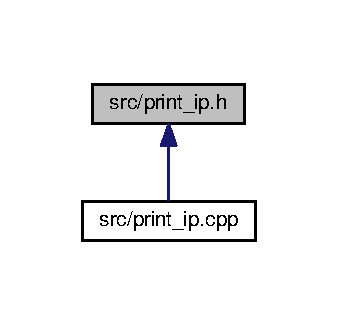
\includegraphics[width=162pt]{print__ip_8h__dep__incl}
\end{center}
\end{figure}
\subsection*{Namespaces}
\begin{DoxyCompactItemize}
\item 
\hyperlink{namespaceflaber}{flaber}
\end{DoxyCompactItemize}
\subsection*{Functions}
\begin{DoxyCompactItemize}
\item 
{\footnotesize template$<$typename Char\-T $>$ }\\void \hyperlink{namespaceflaber_ac2e2220e0b43c7179450485776033a25}{flaber\-::print\-\_\-ip} (std\-::basic\-\_\-ostream$<$ Char\-T $>$ \&os, const std\-::basic\-\_\-string$<$ Char\-T $>$ \&ip)
\item 
{\footnotesize template$<$template$<$ typename, typename $>$ class Container\-T, typename Value\-T , typename Alloc\-T , typename  = std\-::enable\-\_\-if\-\_\-t$<$!is\-\_\-char\-\_\-v$<$\-Value\-T$>$, Value\-T$>$$>$ }\\void \hyperlink{namespaceflaber_a0a0f3ac76aaf479fde049bb26f0930ef}{flaber\-::print\-\_\-ip} (std\-::ostream \&os, const Container\-T$<$ Value\-T, Alloc\-T $>$ \&t)
\item 
{\footnotesize template$<$typename Char\-T , size\-\_\-t N$>$ }\\void \hyperlink{namespaceflaber_a899f2a8340371796390a26c56bd257c0}{flaber\-::print\-\_\-ip} (std\-::ostream \&os, Char\-T(\&arr)\mbox{[}N\mbox{]})
\item 
{\footnotesize template$<$class Int\-T , typename  = std\-::enable\-\_\-if\-\_\-t$<$std\-::is\-\_\-integral\-\_\-v$<$\-Int\-T$>$, Int\-T$>$$>$ }\\void \hyperlink{namespaceflaber_aa6c37128a4f8005fe33124a175e5df4e}{flaber\-::print\-\_\-ip} (std\-::ostream \&os, Int\-T ip)
\item 
{\footnotesize template$<$class... T\-Params$>$ }\\void \hyperlink{namespaceflaber_a2cd40a0efb0b9101246e8dcb11c6d18e}{flaber\-::print\-\_\-ip} (std\-::ostream \&os, const std\-::tuple$<$ T\-Params...$>$ \&tuple)
\end{DoxyCompactItemize}

%--- End generated contents ---

% Index
\newpage
\phantomsection
\addcontentsline{toc}{chapter}{Index}
\printindex

\end{document}
